\begin{itemize}
\item{Approach}

\tab Our approach was to try different classifier and try and compare which one of those works better for the given dataset of heart disease. The classifiers that we have compared are Linear SVM, Non-linear SVM and Stratified K-Mean on the given vector representation of Cleveland dataset. For our experimental purposes, we have divided our experiment into 2 problems. For both problems, we try to run our classifiers for 60/40 and 80/20 splits where we use 60 per cent and 80 per cent for training our classifiers and 40 per cent  and 20 percent for testing their predictions respectively. Cleveland dataset  has 303 instances and 14 attributes. Our first step is to apply dimensionality reduction and for that purpose we have use Principal Component Analysis (PCA) with 5 components. Once the PCA has been applied on the original X value where X is the feature set, our feature set is reduced to X-new which is a vector representation of 303 samples x 5 features.  First, we try out 60/40 split of X-new where 60 per cent of X-new is used to train the SVM classifier and 40 per cent of X-new is used to test. Similarly, next we try 80/20 split of X-new, which is problem 1 of our experiment. \\

\item{Problem 1}

\tab We classify data using a Linear SVM and predict likelihood of disease belonging to a particular class of severity ranging from 1 to 4 i.e. least to most severe with value of C=0.001. Here, C is the penalty that the classifier incurs every time there is a misclassification that takes place so job of the classifier is to incur penalty as minimal as possible while classifying data in order to keep cost of classification at minimum. In order to check if other type of classifiers work better for this dataset than Linear SVM, we use a RBF i.e. non-linear kernel for the SVM classifier and classify data keeping value of C same. Similarly as last part of our problem 1, we use Stratified k-fold cross validation with 5 folds with a RBF kernel and keeping value of C same as for above classifiers in our search to find which classifier works better for this dataset. The results for this have been shown below in Fig 1 below. \\

\item{Problem 2}

\tab For problem-2 of our experiment, we go a step further by predicting absence (zero) or presence (non-zero) of heart disease. This is possible because we group all severity classes (1 to 4) together which mean that a non-zero would indicate presence of heart disease and a zero would indicate absence of heart disease. Problem-2 of the experiment follows same procedure as that of problem-1. First step is dimensionality reduction for which we use PCA with 5 components that picks best 5 components out of 14 attributes. Now what we get is a vector representation as we obtained in problem-1, which basically implies 303 samples x 5 features. For problem-2, we use an 80/20 split where 80 per cent of data is used to train classifier and 20 per cent is used to test. Now, we follow the same procedure as we did for problem-1 we apply 3 classifiers i.e. Linear SVM, Non-Linear SVM with RBF kernel and Stratified k-means cross validation with 5 folds, all for a value of C=0.001. The results are shown in fig.2. \\

\item{Results}

\begin{center}
  	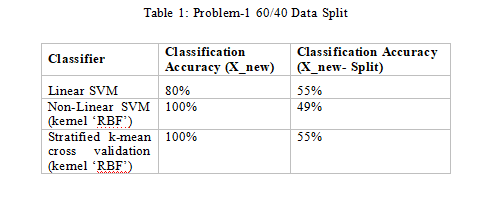
\includegraphics[scale=0.8]{tabel1.png}
\end{center}

\begin{center}
  	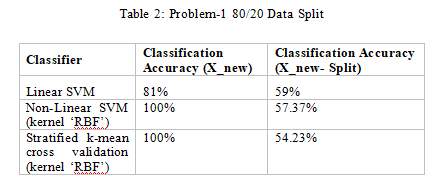
\includegraphics[scale=0.8]{tabel2.png}
\end{center}

\begin{center}
  	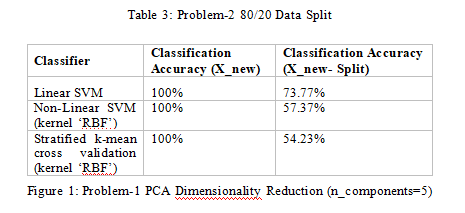
\includegraphics[scale=0.8]{tabel3.png}
\end{center}

\begin{center}
  	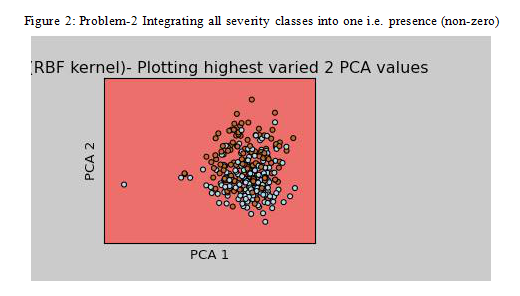
\includegraphics[scale=0.8]{rezultat1.png}
\end{center}

\item{Conclusion}

\tab Based on the results shown above and experiments performed, it is evident that input data plays an important role in prediction along with machine learning techniques. As is seen in the dataset, provided, we have labels from 0 to 4 where the labels of 4 are hardly 13 and when we split the data into train and test, the number become very less which is nothing but noise and can be totally removed from the dataset by using filtering techniques and hence the linear model will be available to predict the outcome much better with absence of noise. Moreover, PCA has again proven that we can get rid of similar feature set and still obtain predictions with great efficiency. Moreover, we have conducted tests using non linear RBF kernel which is a normal first choice and then validating against linear SVC kernel which outperformed RBF in split case. Most importantly, the above experiment not only helped us in predicting the outcome but also gave us valuable insights about the nature of data, which can be used in future to train our classifiers in a much better way. \\

\tab All source file can be founded  \href{https://github.com/diwakar02/Heart-Disease-Prediction-using-Machine-Leaning}{here.}\\

\end{itemize}